% !TeX program = pdflatex
% Main manuscript for submission to Frontiers of Computer Science.
\documentclass[research]{fcs}

\usepackage{subfig}
\usepackage{algorithm}
\usepackage{algorithmicx}
\usepackage{algpseudocode}
\usepackage{listings}
\usepackage{tikz}
\usetikzlibrary{arrows.meta,calc,fit,positioning,shapes.geometric}

\title{TRIDENT: GPU-Accelerated EKF Positioning for Downhole Traction Robots}
\shorttitle{TRIDENT: GPU-Accelerated EKF Positioning for Downhole Traction Robots}

% TODO: Replace the author, affiliation, and correspondence placeholders.
\author[1,+]{First~Author}
\author[1]{Second~Author}
\address[1]{Department, University, City Postal Code, China}
\corremail{corresponding.author@example.com}

\fcssetup{
  received = {month dd, yyyy},
  accepted = {month dd, yyyy},
  article-id = {1},
  first-page = {1},
}

\begin{abstract}
Extended Kalman filter (EKF)-based multi-sensor fusion underpins positioning algorithms for robots that operate without reliable external positioning. In simulations of a downhole traction robot in a cased horizontal well, the estimator processes a long sensor sequence through tightly dependent SINS propagation and EKF correction steps. Its small matrices and fine-grained operators form a latency-bound GPU workload: a direct tensor implementation expands each filter step into about 531 dependent kernels, so dispatch, synchronization, and recurrent-state movement can dominate arithmetic and leave most streaming multiprocessors idle. We present \textsc{Trident}, a three-axis GPU acceleration framework for this workload. First, a Triton whole-scan kernel fuses the complete recursive trajectory, keeps the recurrent navigation and filter state on chip, and replaces the general innovation solve with an analytical small-matrix inverse. Second, component-aware specialization separates the precision of sensor input, recurrent computation, and dot products; full-trajectory screening shows that fp16 sensor input is safe, that bfloat16 input and fp16 recurrent storage are unsafe for the long-horizon filter, and that TF32 products add measurable deviation at little or no gain in throughput, so the adopted plan keeps IEEE dot products. Third, independent simulation trajectories are mapped to CUDA blocks to expose batch-level parallelism without changing the temporal order within each filter. Across two GPU architectures (an Ampere A100 and a Hopper-class H20), \textsc{Trident} achieves up to roughly $3\times10^{4}\times$ the naive GPU baseline throughput via multi-trajectory batching, with negligible accuracy loss relative to the fp64 reference. These results show how execution granularity, numerical representation, and outer-loop parallelism can be coordinated for long-horizon recursive state-estimation simulation.
\end{abstract}
\keywords{}
\ExplSyntaxOn
\tl_clear:N \l__fcs_keywords_tl
\ExplSyntaxOff

\begin{document}

\section{Introduction}
\label{sec:introduction}

Embodied artificial intelligence (AI) is extending autonomous machines from structured, instrumented spaces into physical environments with uncertain contacts, limited visibility, and unreliable external positioning~\cite{liu2025embodied-survey}. A robot must maintain an estimate of its pose, velocity, and internal state while it perceives the environment, plans motion, and applies control. Deep-space vehicles, subterranean platforms, legged robots~\cite{he2024legged-state,ou2024leg-kilo}, and autonomous vehicles use different sensors and motion models, yet their local state-estimation loops repeatedly propagate inertial information and correct it with intermittent observations through recursive Bayesian estimation. The quality and timeliness of this loop determine how reliably the rest of the perception--action system can operate.

This requirement is especially visible in embodied-AI systems~\cite{embodied-ai-survey}. Humanoids and quadrupeds combine inertial, kinematic, contact, and visual measurements at high update rates; a local extended Kalman filter (EKF) or error-state filter often provides the high-rate inertial-propagation and measurement-correction layer even when a separate mapping system supplies global consistency. Consistent fusion of leg kinematics and inertial measurements has been demonstrated for legged robots~\cite{bloesch2012}, while the DARPA Subterranean Challenge shows how localization, mapping, and navigation must remain tightly coupled when robots operate in underground environments~\cite{cerberus2022}. Such robots increasingly depend on large simulation campaigns that vary contact conditions, sensor noise, terrain, and control parameters. GPU-native simulators such as Isaac Gym execute thousands of robot environments concurrently~\cite{isaacgym2021}, so every repeated state-estimation loop in the pipeline must sustain higher throughput.

Downhole traction robots provide a concrete and demanding instance of this broader embodied-autonomy problem. These robots actively convey coiled tubing, toolstrings, and attached tools through highly deviated and horizontal wells, where gravity, friction, and long constrained passages make passive delivery unreliable. Recent field deployments have demonstrated their use in horizontal-well intervention, logging, perforation, and zonal-isolation operations~\cite{he2020downhole-tractor,chawla2024tractor-glide}. As illustrated in \Cref{fig:downhole-tractor}, a surface unit deploys the toolstring through the wellbore while the tractor provides active conveyance along the horizontal section. In the cased horizontal well considered in this study, high temperature and pressure, corrosion, deposits, local deformation, and obstructions can perturb wheel--wall contact and induce slip or short-lived odometry disturbances. Reliable operation therefore requires continuous fusion of inertial and traction measurements through a strapdown inertial navigation system (SINS) supporting an error-state extended Kalman filter, to estimate the robot state and suppress accumulated drift. Before deployment, large simulation campaigns are needed to evaluate sensor noise, slip events, obstacle-induced disturbances, and filter parameters over long trajectories, making downhole traction robot positioning not only a state-estimation problem but also a computationally intensive simulation workload.

\begin{figure}[!t]
  \centering
  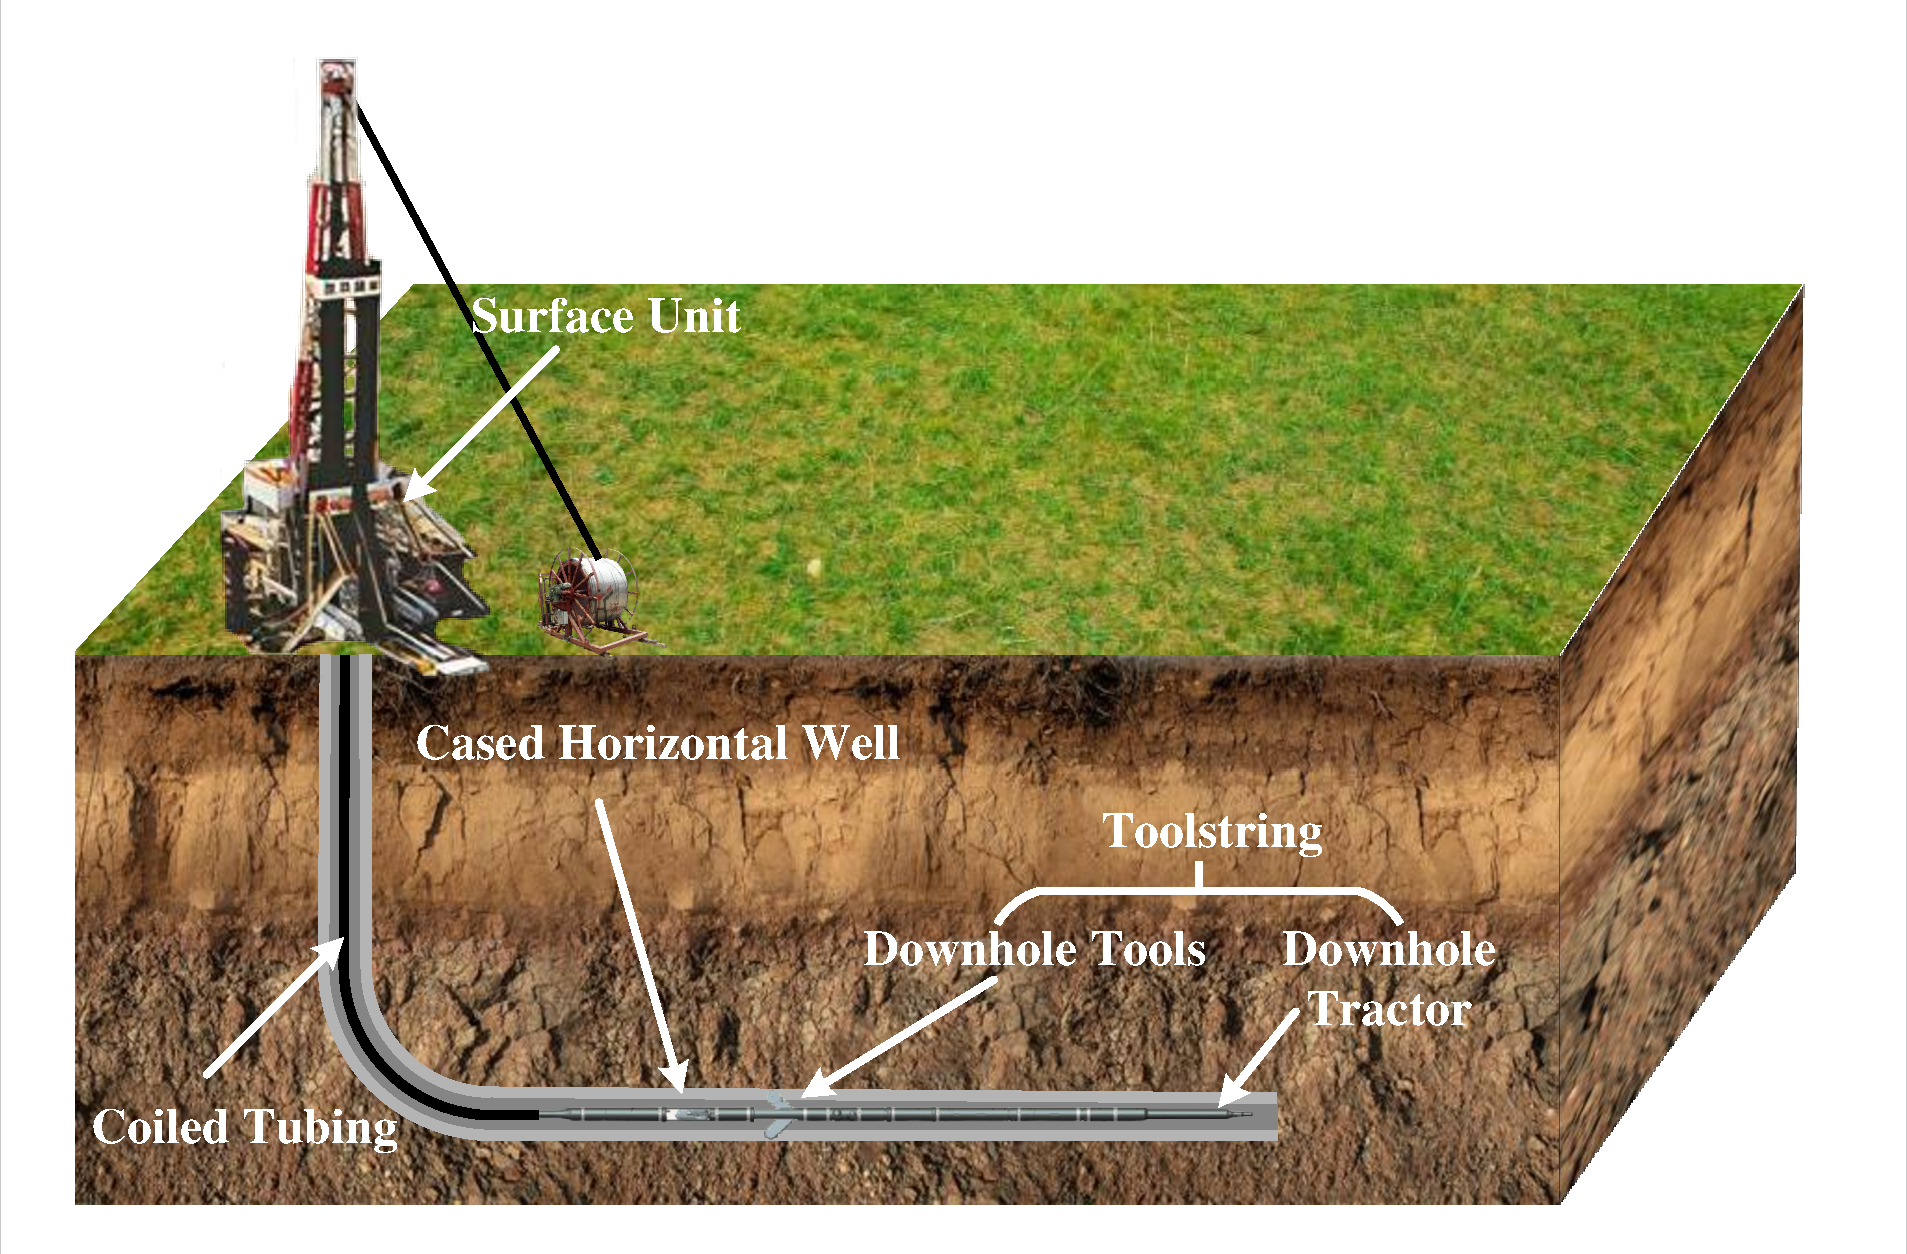
\includegraphics[width=\linewidth]{figures/1-intro-robot.pdf}
  \caption{Schematic of a downhole traction robot conveying a toolstring into the horizontal section of an oil or gas well.}
  \label{fig:downhole-tractor}
\end{figure}

The resulting estimator has an execution pattern that differs from the large, throughput-oriented matrix workloads commonly used to showcase GPUs. Although the simulation campaigns described above are throughput-hungry, each estimator update is a small numerical operation embedded in a long dependency chain, and a direct tensor implementation fragments the computation into many fine-grained device operations. Repeated launches, synchronization, and movement of recurrent state can dominate arithmetic, leaving much of the accelerator underutilized and causing a straightforward GPU port to underperform a CPU implementation. These characteristics motivate an implementation study centered on launch overhead, on-chip state locality, numerical precision, and independent trajectories available at the simulation level.

We develop \textsc{Trident}, a GPU acceleration framework for this workload. It composes three complementary optimizations---operator fusion, component-aware mixed precision, and multi-trajectory batching---which target the dispatch, numerical, and device-occupancy bottlenecks above. The main contributions are as follows:

\begin{itemize}
  \item We diagnose the execution behavior of SINS/EKF simulation and develop a progressive fusion path culminating in a single fused whole-scan Triton kernel that keeps the recurrent filter state on chip and executes a complete trajectory with minimal device dispatch.
  \item We establish a component-aware precision strategy for recursive filtering and evaluate the performance and long-horizon accuracy of fp64 and fp32 recursive arithmetic, fp16 and bfloat16 sensor input, and IEEE versus TensorFloat-32 dot products, including failure cases caused by error accumulation.
  \item We map independent trajectories to CUDA blocks and derive a scaling model that relates batch throughput to accelerator occupancy and register pressure, enabling high-throughput Monte Carlo and parameter-sweep simulation.
\end{itemize}

The remaining sections of this paper are organized as follows. \Cref{sec:background} introduces the positioning model and its computational structure. \Cref{sec:motivation} presents the profiling evidence and optimization requirements. \Cref{sec:methodology} describes the \textsc{Trident} framework. \Cref{sec:evaluation} evaluates performance, accuracy, and scalability. \Cref{sec:related-work} discusses related work and \Cref{sec:conclusion} concludes the paper.

\section{Background}
\label{sec:background}

\subsection{Downhole Traction Robot Positioning}
\label{subsec:positioning-background}

Downhole traction robots provide the active conveyance on which intervention in highly deviated and horizontal wells depends. The deployment configuration in \Cref{fig:downhole-tractor} shows the tractor moving with the toolstring while its drive elements maintain contact with the well wall. This study considers operation inside a cased horizontal well, where the available space is narrow and absolute positioning signals are generally unavailable. High temperature and pressure, corrosion, deposits, local deformation, and obstructions can change the contact conditions between the robot and the casing. These effects can introduce wheel slip and short-duration disturbances while the robot performs intervention, logging, perforation, or other downhole operations. A positioning system must therefore maintain a local state estimate over a long constrained motion and remain useful when an individual measurement becomes unreliable.

The simulated platform uses a three-axis inertial measurement unit (IMU) and two wheel odometers. Gyroscope and accelerometer measurements support high-rate propagation of attitude, velocity, and position, but their biases cause the propagated solution to drift over time. The odometers provide an independent estimate of traveled distance, which the estimator folds into a single displacement measurement that corrects the propagated drift, while disagreement between the two odometers or between odometry and inertial propagation provides a signal for detecting local disturbances. The fusion system uses these complementary measurements in a local navigation frame whose origin and initial attitude are set during initialization.

The casing geometry supplies additional information about feasible robot motion. During nominal traction, displacement is dominated by the direction of the well axis, whereas sustained lateral or radial velocity is inconsistent with the confined workspace. These motion constraints improve local observability when absolute position is unavailable. They cannot, however, be treated as uniformly reliable: wheel slip, asymmetric traction, and obstacle contact can produce transient measurements that violate the nominal motion pattern. The estimator must therefore combine continuous inertial propagation with measurement selection, using the available odometry information without allowing a short-lived contact disturbance to corrupt the full trajectory.

\subsection{SINS/EKF Fusion Model}
\label{subsec:ekf-model}

The simulation follows a SINS with an error-state extended Kalman filter. At sample $k$, the SINS first updates the quaternion attitude from the angular-rate measurement, converts the measured specific force from the body frame to the navigation frame, subtracts gravity, and integrates velocity and position. Quaternion normalization is applied after each update to keep the attitude representation bounded.

The SINS state is maintained as a nominal navigation solution, while the EKF represents only small deviations from that solution. This error-state formulation separates the nonlinear integration of attitude and motion from the locally linear uncertainty update. It also supports closed-loop correction: after the EKF estimates the navigation errors, the nominal position, velocity, and attitude are corrected and the corresponding error coordinates are reset. Sensor biases remain part of the estimated state because even small bias errors can accumulate during a long period without an external position reference.

The EKF estimates the error of the nominal SINS state. Its 15-dimensional error vector is
\begin{equation}
  \mathbf{x}_k =
  [\delta\mathbf{p}_k^{\mathsf T},
   \delta\mathbf{v}_k^{\mathsf T},
   \boldsymbol{\phi}_k^{\mathsf T},
   \boldsymbol{\varepsilon}_k^{\mathsf T},
   \boldsymbol{\nabla}_k^{\mathsf T}]^{\mathsf T}
  \in \mathbb{R}^{15},
  \label{eq:error-state}
\end{equation}
where the five three-dimensional components represent position error, velocity error, attitude error, gyroscope bias, and accelerometer bias, respectively.

The linearized transition matrix is constructed from the current attitude, specific force, angular rate, and sampling interval. The covariance and error state are then propagated and corrected through the standard EKF prediction and measurement update:
\begin{align}
  \mathbf{x}_{k}^{-} &= \mathbf{F}_k\mathbf{x}_{k-1}, \\
  \mathbf{P}_{k}^{-} &= \mathbf{F}_k\mathbf{P}_{k-1}\mathbf{F}_k^{\mathsf T}+\mathbf{Q}_k, \\
  \mathbf{K}_k &= \mathbf{P}_{k}^{-}\mathbf{H}_k^{\mathsf T}
  (\mathbf{H}_k\mathbf{P}_{k}^{-}\mathbf{H}_k^{\mathsf T}+\mathbf{R}_k)^{-1}, \\
  \mathbf{x}_k &= \mathbf{x}_{k}^{-}+\mathbf{K}_k
  (\mathbf{z}_k-\mathbf{H}_k\mathbf{x}_{k}^{-}), \\
  \mathbf{P}_k &= (\mathbf{I}-\mathbf{K}_k\mathbf{H}_k)\mathbf{P}_{k}^{-}.
  \label{eq:ekf-update}
\end{align}

Here, $\mathbf{F}_k$ is the linearized state-transition matrix, $\mathbf{P}_k$ is the error covariance, and $\mathbf{Q}_k$ models process uncertainty. The observation matrix $\mathbf{H}_k$ maps the error state into the currently available measurement space, while $\mathbf{R}_k$ represents measurement uncertainty. The matrix inverted in the gain calculation is the innovation covariance. Although its dimension is small in this application, its value changes with the propagated covariance and the accepted measurement set at every sample.

When the consistency test accepts both wheel-odometer measurements, the measurement model combines the odometry displacement with the lateral and radial velocity constraints. If an odometer reading or a velocity constraint is judged unreliable, the update uses only the remaining reliable components. Because the corrected errors are fed back into the nominal state at every sample, each update depends on the state and covariance produced at the previous sample.

\subsection{Computational Characteristics}
\label{subsec:workload-characteristics}

The overall computation is summarized in \Cref{fig:computational-flow}. The resulting workload is a long sequential scan of sensor samples. Each step combines quaternion and vector operations with covariance propagation, a small innovation calculation, and several products involving matrices whose logical dimensions are no larger than $15\times15$. The arithmetic intensity of an individual step is consequently modest, while the recurrent state and covariance must remain available for the next step. Temporal parallelism within one trajectory is therefore limited by the estimator semantics.

\begin{figure}[!t]
  \centering
  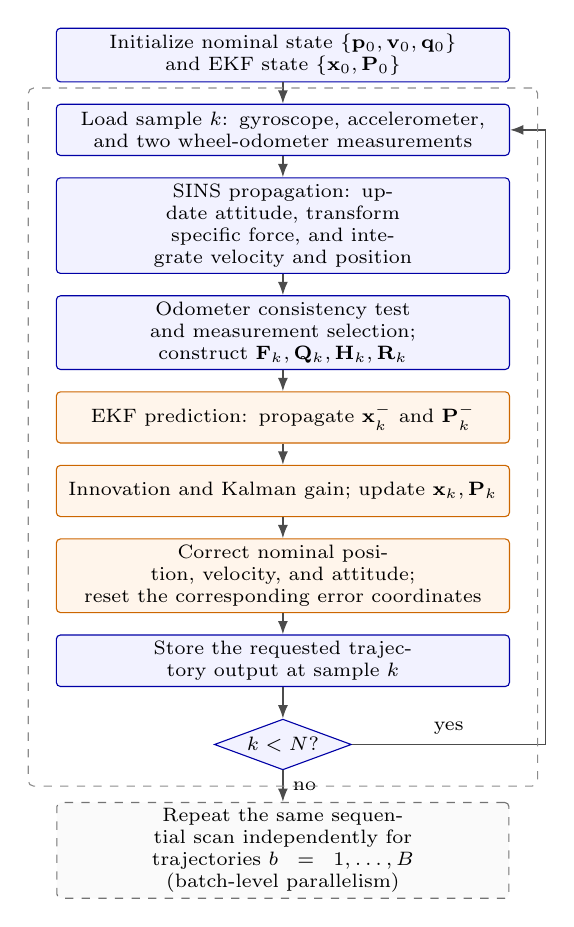
\begin{tikzpicture}[
      node distance=2.7mm,
      font=\scriptsize,
      flow/.style={draw=blue!65!black, rounded corners=1.5pt,
        fill=blue!5, align=center, minimum height=6.5mm,
        text width=5.6cm, inner sep=2.2pt},
      update/.style={flow, draw=orange!80!black, fill=orange!8},
      decision/.style={diamond, draw=blue!65!black, fill=blue!5,
        align=center, aspect=2.7, inner sep=1.2pt},
      note/.style={draw=black!55, dashed, rounded corners=1.5pt,
        fill=black!2, align=center, minimum height=6mm,
        text width=5.6cm, inner sep=2pt},
      arrow/.style={-{Latex[length=1.7mm]}, semithick, draw=black!70}
    ]
    \node[flow] (init) {Initialize nominal state $\{\mathbf{p}_0,\mathbf{v}_0,\mathbf{q}_0\}$\\and EKF state $\{\mathbf{x}_0,\mathbf{P}_0\}$};
    \node[flow, below=of init] (load) {Load sample $k$: gyroscope, accelerometer,\\and two wheel-odometer measurements};
    \node[flow, below=of load] (sins) {SINS propagation: update attitude, transform\\specific force, and integrate velocity and position};
    \node[flow, below=of sins] (select) {Odometer consistency test and measurement selection;\\construct $\mathbf{F}_k,\mathbf{Q}_k,\mathbf{H}_k,\mathbf{R}_k$};
    \node[update, below=of select] (predict) {EKF prediction: propagate $\mathbf{x}_k^{-}$ and $\mathbf{P}_k^{-}$};
    \node[update, below=of predict] (correct) {Innovation and Kalman gain; update $\mathbf{x}_k,\mathbf{P}_k$};
    \node[update, below=of correct] (feedback) {Correct nominal position, velocity, and attitude;\\reset the corresponding error coordinates};
    \node[flow, below=of feedback] (store) {Store the requested trajectory output at sample $k$};
    \node[decision, below=4.0mm of store] (next) {$k<N$?};
    \node[note, below=4.0mm of next] (batch) {Repeat the same sequential scan independently for\\trajectories $b=1,\ldots,B$ (batch-level parallelism)};

    \draw[arrow] (init) -- (load);
    \draw[arrow] (load) -- (sins);
    \draw[arrow] (sins) -- (select);
    \draw[arrow] (select) -- (predict);
    \draw[arrow] (predict) -- (correct);
    \draw[arrow] (correct) -- (feedback);
    \draw[arrow] (feedback) -- (store);
    \draw[arrow] (store) -- (next);
    \draw[arrow] (next) -- node[right, font=\scriptsize] {no} (batch);
    \coordinate (returntop) at ([xshift=4.5mm]load.east);
    \coordinate (returnbottom) at (next.east -| returntop);
    \draw[arrow] (next.east) -- node[above, font=\scriptsize] {yes}
      (returnbottom) |- (load.east);

    \node (scanbox) [draw=black!45, dashed, rounded corners=2pt,
      fit=(load)(next), inner xsep=3.5mm, inner ysep=2.0mm] {};
  \end{tikzpicture}
  \caption{Overall computational flow of the SINS/EKF positioning simulation. Operations within one trajectory follow a loop-carried dependency, whereas different trajectories have independent recurrent states and can be evaluated in parallel.}
  \label{fig:computational-flow}
\end{figure}

The covariance alone contains 225 logical elements, yet this state is still too small to provide the spatial parallelism of a large dense matrix operation. Moreover, the matrices used at a given sample are assembled from the current navigation state and measurement-validity decision rather than reused unchanged across the sequence. The workload therefore alternates small matrix products with quaternion normalization, coordinate transforms, scalar tests, and feedback operations. Its defining feature is not the cost of any individual operator, but the repeated execution of this heterogeneous operator chain under a loop-carried dependency.

The simulation nevertheless exposes a second form of parallelism. Trajectories generated with different noise realizations, obstacle configurations, or filter parameters do not share state and can be evaluated independently. Increasing the trajectory length adds sequential work, whereas increasing the number of trajectories adds independent work. The workload thus combines a sequential dependency along each trajectory with batch-level independence across trajectories. This combination defines the execution target for the optimization methods developed in the remaining sections of the paper. For fixed-shape kernel implementations, the logical filter matrices may be stored in padded $16\times16$ tiles without changing the 15-state model.

\section{Motivation}
\label{sec:motivation}

\subsection{Fine-Grained EKF Execution Is Latency-Bound}
\label{subsec:motivation-latency}

The CPU fp64 implementation processes approximately 1,866 filter steps per second and serves as the numerical reference; its representative characteristics are summarized in \Cref{tab:baseline-characteristics}. Moving the same tensor-level computation directly to the GPU does not produce a corresponding speedup. Each EKF step contains a dependent chain of tensor construction, element-wise arithmetic, trigonometric functions, and small matrix operations. The eager implementation expands this modest amount of arithmetic into roughly 531 CUDA kernel launches per step. As a result, dispatch, synchronization, and recurrent-state transfers occupy a substantial part of the execution time.

Device measurements confirm that the baseline is latency-bound. A single trajectory activates only a small portion of the GPU, and its measured SM throughput is approximately $0.27\%$. The launch cost of a general-purpose small-matrix kernel can approach or exceed the cost of its arithmetic. CUDA Graph replay reduces repeated host dispatch, but the captured graph still executes the fine-grained dependent kernels and transfers state between them. These observations motivate a larger execution scope that can preserve recurrent data across filter steps and eliminate fragmented device execution.

\begin{table}[H]
  \centering
  \caption{Representative characteristics of the baseline positioning workload (GPU utilization measured on an H20).}
  \label{tab:baseline-characteristics}
  \begin{tabular}{@{}lr@{}}
    \toprule
    Characteristic & Value \\
    \midrule
    Trajectory length & 166,667 steps \\
    EKF state dimension & 15 \\
    Maximum logical matrix size & $15\times15$ \\
    Naive kernels per step & approximately 531 \\
    CPU fp64 throughput & 1,866 steps/s \\
    Naive GPU SM throughput & approximately 0.27\% \\
    \bottomrule
  \end{tabular}
\end{table}

\subsection{Precision Choices Have Unequal Numerical and Hardware Effects}
\label{subsec:motivation-precision}

Uniformly changing the precision of the estimator overlooks the different roles of its components. Sensor samples are noisy external inputs that are consumed once, whereas position, velocity, attitude, error state, and covariance are carried through the complete trajectory. Rounding in these recurrent quantities can accumulate through repeated propagation and feedback. Accuracy measured for an isolated filter step is therefore insufficient to determine whether a reduced-precision configuration is acceptable over a long simulation.

Lower nominal precision also does not guarantee lower execution time. TensorFloat-32 and Tensor Core paths may require conversion, padding, and scheduling work that is difficult to amortize for the small matrices in this estimator. Storage precision, recurrent arithmetic, and matrix-multiplication mode consequently present different accuracy and performance trade-offs. This behavior motivates component-level precision choices evaluated with both hardware measurements and complete-trajectory numerical error. \Cref{fig:precision-tradeoff} combines the two views for the complete trajectory: throughput (bars) and the per-axis deviation from the all-fp32 reference (lines) share one panel, so accuracy and performance can be read together for each configuration.

We additionally isolate one precision decision at a time over the complete 166,667-step trajectory, while retaining fp32/IEEE arithmetic for all remaining components. As summarized in \Cref{tab:precision-isolation}, fp16 sensor input causes only limited additional error, whereas bfloat16 input substantially amplifies the vertical error. TF32 matrix products introduce a measurable X-axis deviation, and storing the recurrent navigation state in fp16 causes the long-horizon filter to diverge. These outcomes distinguish once-consumed sensor data from values repeatedly propagated through the recursion and motivate the component-aware scheme in \Cref{sec:methodology}.

\begin{table}[H]
  \centering
  \caption{Component-isolation precision study over the full 166,667-step trajectory in the fused scan (\Cref{subsec:kernel-fusion}), measured on an H20. Each row lowers one component while the remaining components use fp32/IEEE arithmetic; values report the per-axis RMSE difference (mm) against the all-fp32 reference.}
  \label{tab:precision-isolation}
  \begin{tabular}{@{}llrr@{}}
    \toprule
    Component & Lowered mode & $\Delta$X (mm) & $\Delta$Z (mm) \\
    \midrule
    Sensor input & fp16 & $0.11$ & $2.19$ \\
    Matrix products & TF32 & $4.82$ & $0.31$ \\
    Sensor input & bfloat16 & $11.01$ & $1005.84$ \\
    Recurrent state & fp16 storage & $280753.72$ & $-0.30$ \\
    \bottomrule
  \end{tabular}
\end{table}

\begin{figure}[!t]
  \centering
  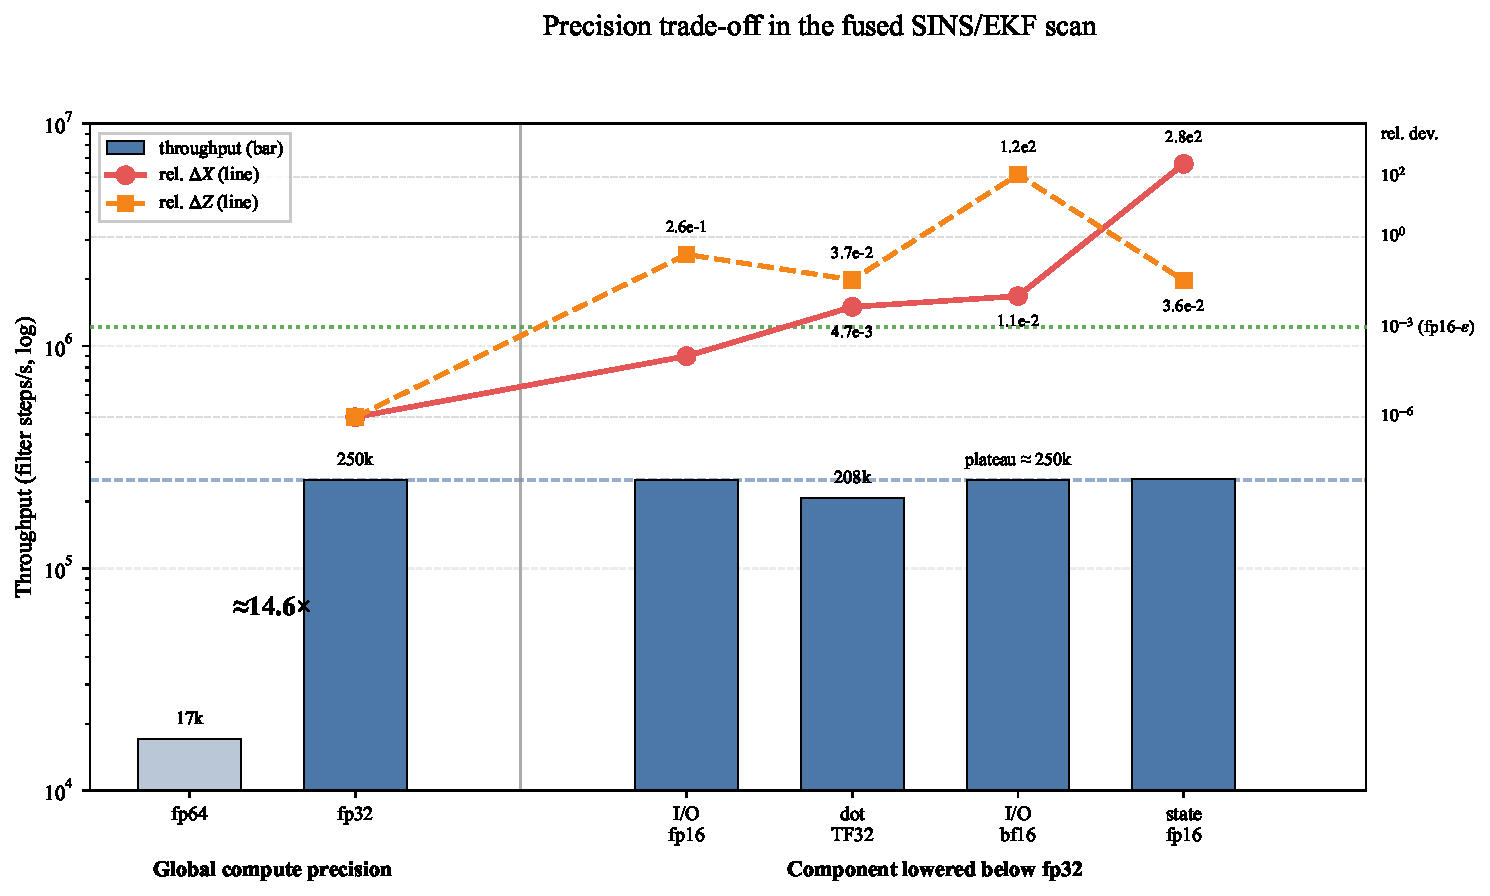
\includegraphics[width=\linewidth]{figures/3-motivation-precision_tradeoff.pdf}
  \caption{Precision trade-off in the fused SINS/EKF scan (\Cref{subsec:kernel-fusion}) over the full 166{,}667-step trajectory, measured on an H20. Bars (lower log axis) report end-to-end throughput, and lines (upper band, log axis) report the relative X/Z positioning deviation against the all-fp32 reference. The $10^{-3}$ line marks an fp16-$\varepsilon$ accuracy grade: bfloat16 sensor input and fp16 recurrent storage cross it and are unsafe for the long-horizon filter, whereas fp16 sensor input remains safely below it. TF32 matrix products sit near the boundary but add measurable deviation for negligible or negative throughput gain, and are consequently excluded by the component-aware plan.}
  \label{fig:precision-tradeoff}
\end{figure}

\subsection{Independent Trajectories Supply Device-Level Parallelism}
\label{subsec:motivation-trajectories}

The state and covariance at time $k$ depend on the result at time $k-1$, which limits temporal parallelism within one trajectory. Increasing the tile size or assigning more threads to an individual small matrix product cannot create work along this dependency chain. Kernel fusion removes dispatch and state-traffic overhead, but it does not change this limit: a single fused trajectory launches one 128-thread block, or four warps. On a Hopper-class H20, this block occupies only one SM at 6.25\% warp occupancy, leaving the device almost entirely idle, as summarized in \Cref{tab:motivation-utilization}. Reducing single-trajectory latency alone therefore cannot fill the GPU.

Simulation campaigns naturally provide an outer parallel dimension. Different noise realizations, obstacle configurations, and filter parameters produce independent trajectories with no shared recurrent state. Mapping these trajectories to separate blocks preserves the original update order within every filter while increasing aggregate device utilization. Scaling eventually becomes limited by the number of SMs and by register-constrained block residency. Together, the three observations above lead to whole-scan kernel fusion, component-aware precision, and multi-trajectory parallelism, which are developed in the next section.

\begin{table}[H]
  \centering
  \caption{Measured utilization for one fused fp32 trajectory on an H20. The kernel uses one 128-thread block per trajectory.}
  \label{tab:motivation-utilization}
  \begin{tabular}{@{}lr@{}}
    \toprule
    Characteristic & Value \\
    \midrule
    Grid / block size & $(1,1,1)$ / 128 threads (4 warps) \\
    SMs hosting the block & 1 of 78 \\
    Achieved occupancy & 6.25\% (4 / 64 warps) \\
    Device SM throughput & approximately 0.27\% \\
    \bottomrule
  \end{tabular}
\end{table}

\section{Methodology}
\label{sec:methodology}

\subsection{Overview}
\label{subsec:method-overview}

\textsc{Trident} models each positioning trajectory as a recursive scan over $N$ sensor samples. At step $k$, the scan reads the current IMU and odometer measurements, propagates the nominal SINS state, performs EKF prediction and correction, feeds the estimated error back to the nominal state, and carries the updated navigation state and covariance to step $k+1$. A batch of $B$ simulations adds an outer trajectory dimension to the input and output tensors; the recurrent state remains private to each trajectory.

\Cref{fig:design-overview} summarizes three complementary optimizations. First, whole-scan fusion encloses the complete time loop in one kernel, retains recurrent state on chip, and specializes the small-matrix operations on the critical path. Second, component-aware precision specialization assigns representations according to numerical role and selects a compile-time precision plan under a trajectory-level error constraint. Third, multi-trajectory mapping assigns independent scans to separate CUDA blocks, exposing device-wide parallelism subject to register-residency limits. The three axes target different bottlenecks---dispatch and data movement, arithmetic and storage cost, and insufficient device-level parallelism---and can therefore be composed.

These transformations preserve the SINS/EKF equations and the order of propagation, measurement selection, prediction, correction, and feedback within every trajectory. We use the CPU fp64 implementation as the semantic reference, compare complete output trajectories rather than isolated steps, and repeat identical trajectories across blocks to detect accidental state sharing. \Cref{sec:evaluation} reports the corresponding performance and accuracy results.

\begin{figure}[!t]
  \centering
  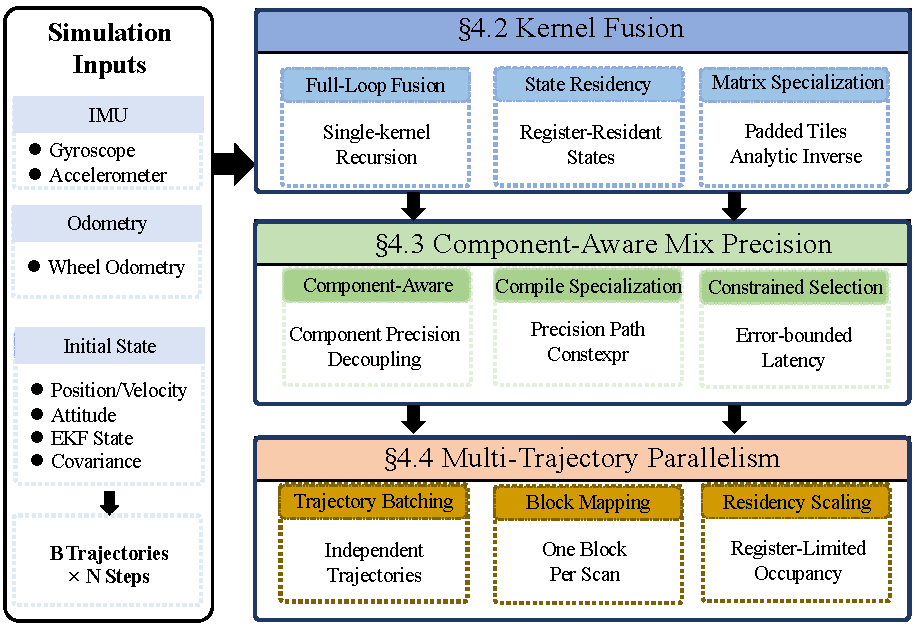
\includegraphics[width=\linewidth]{figures/4-method-overview.pdf}
  \caption{Overview of \textsc{Trident}. Kernel fusion retains recurrent state on chip, component-aware mixed precision selects numerically safe precision paths, and block-level trajectory mapping exposes device-wide parallelism.}
  \label{fig:design-overview}
\end{figure}

\subsection{From Fragmented Operators to a Fused Recursive Scan}
\label{subsec:kernel-fusion}

\Cref{fig:fusion-path}(a) contrasts the eager and whole-scan fusion boundaries. In the eager implementation, one filter step expands into approximately 531 dependent kernels. Recurrent values therefore cross kernel boundaries and return to HBM hundreds of times per step, even though the next operation immediately consumes them.

We first regularize the step for static compilation. Scalar tensor construction, host-visible scalar access, and dynamic concatenation are replaced with device-side expressions. The observation shapes that arise when the consistency test rejects a component are unified into one fixed three-dimensional representation; a large variance suppresses the corresponding Kalman gain without changing the matrix shape. CUDA Graph replay then removes repeated host dispatch, but the captured graph still contains the fine-grained kernels and their recurrent-state transfers. Whole-scan fusion removes this remaining boundary by placing all $N$ steps inside one Triton program. A single host launch enters the scan, and the loop preserves the original update order while reusing state across iterations.

\begin{figure}[!t]
  \centering
  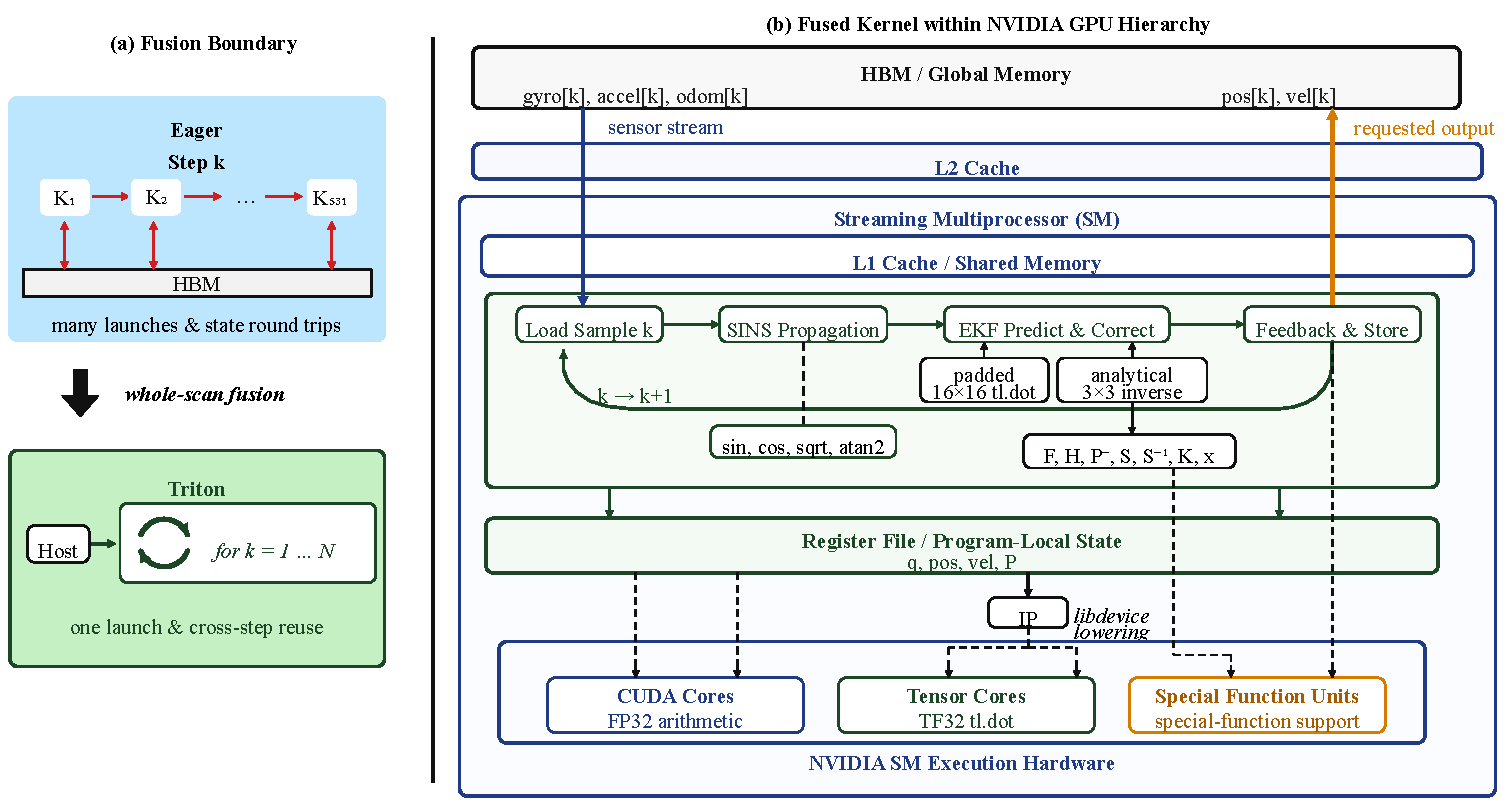
\includegraphics[width=\linewidth]{figures/4-method-fusion.pdf}
  \caption{Whole-scan fusion and its GPU mapping. (a) Fusion replaces hundreds of eager kernels per step with one Triton launch for the full trajectory. (b) The fused program streams sensor samples and requested outputs through HBM while retaining recurrent state in registers and mapping matrix and special-function operations to the corresponding SM execution units.}
  \label{fig:fusion-path}
\end{figure}

\Cref{fig:fusion-path}(b) shows the resulting data path. At iteration $k$, the program streams only the current gyroscope, accelerometer, and odometer samples through L2 and the SM cache hierarchy. It performs SINS propagation, EKF prediction and correction, and feedback before advancing to $k+1$. Only the requested position and velocity outputs are written to global memory. The quaternion, position, velocity, error state, and covariance remain program-local, so the loop-carried dependency passes through the register file instead of intermediate global-memory tensors.

Two in-kernel transformations make the loop static and self-contained. First, masked $16\times16$ tiles store the logical 15-state filter matrices, providing a common layout for transition, covariance, observation, and gain products. The compile-time dot-product mode lowers these products to either CUDA-core IEEE arithmetic or Tensor Core TF32 operations. Second, the kernel computes the inverse of the $3\times3$ innovation covariance from its adjugate and determinant, avoiding a general solver and its synchronization point. SINS transcendental functions, including sine, cosine, square root, and arctangent, follow the device special-function path. The mapping in \Cref{fig:fusion-path}(b) thus combines one fusion boundary, register-resident recurrence, and hardware-specific micro-operations to reduce dispatch, synchronization, and HBM traffic on the latency-bound critical path.

\subsection{Component-Aware Precision Specialization}
\label{subsec:mixed-precision}

Uniform precision ignores the different numerical roles within the scan. Sensor samples are noisy, once-consumed inputs, whereas position, velocity, attitude, error state, and covariance recur across the complete trajectory and can accumulate rounding error. Small matrix products introduce a third choice because TensorFloat-32 (TF32) changes the multiplication path without changing the surrounding storage type. We therefore treat input storage, recurrent arithmetic, and dot-product mode as independent dimensions.

The fused kernel exposes these dimensions as three compile-time parameters. $\mathit{DT}_{\mathrm{IO}}$ specifies the stored type of IMU and odometer samples, which are converted on load to the internal arithmetic type $\mathit{DT}$. The latter governs quaternion normalization, SINS integration, EKF prediction, covariance update, and feedback. $\mathit{IP}$ selects the Triton dot-product mode, distinguishing IEEE and TF32 execution. Because all three parameters are compile-time constants, each combination produces a branch-free specialized kernel. We define a precision plan as $P=(\mathit{DT}_{\mathrm{IO}},\mathit{DT},\mathit{IP})$ over the candidate sets in \Cref{tab:precision-design}. For this workload the plan selected by \Cref{eq:precision-accept} is, as the evaluation reports, the all-fp32/IEEE plan---fp32 sensor input, fp32 recursive arithmetic, and IEEE dot products---while TF32 products are excluded on accuracy and hardware grounds.

\begin{table}[H]
  \centering
  \caption{Precision dimensions exposed by the fused implementation.}
  \label{tab:precision-design}
  \begin{tabular}{@{}lll@{}}
    \toprule
    Component & Candidates & Treatment \\
    \midrule
    Sensor input & fp16, bf16, fp32 & cast to $\mathit{DT}$ \\
    Recursive computation & fp32, fp64 & retain across steps \\
    Small matrix products & IEEE, TF32 & $\mathit{IP}$ specialization \\
    Validation reference & fp64 & CPU trajectory \\
    \bottomrule
  \end{tabular}
\end{table}

We screen each plan over the complete trajectory rather than an isolated filter step. Let $\mathbf{p}^{P}_{0:N}$ be the position trajectory produced by plan $P$, and let $\mathbf{p}^{\mathrm{ref}}_{0:N}$ be the CPU fp64 trajectory. The precision-induced deviation is
\(
  \delta_{P}=\mathrm{RMSE}(\mathbf{p}^{P}_{0:N},\mathbf{p}^{\mathrm{ref}}_{0:N}).
\)
Evaluating all $N$ steps exposes errors that emerge only after repeated integration or covariance propagation. We separately define the irreducible model error as $\varepsilon_{\mathrm{model}}=\mathrm{RMSE}(\mathbf{p}^{\mathrm{ref}}_{0:N},\mathbf{p}^{\mathrm{truth}}_{0:N})$. For a dimensionless tolerance $\alpha$, plan $P$ is acceptable when
\begin{equation}
  \delta_{P}\le\alpha\,\varepsilon_{\mathrm{model}},
  \label{eq:precision-accept}
\end{equation}
so that numerical error introduced by the precision plan remains small relative to the model error already present in the fp64 reference. This criterion separates numerical acceptance from hardware behavior: $\mathit{DT}_{\mathrm{IO}}$ changes input storage and bandwidth, $\mathit{DT}$ changes recurrent arithmetic and state representation, and $\mathit{IP}$ changes dot-product execution. Among the acceptable plans, we select the one with the lowest critical-path latency $\tau_{P}$, breaking ties by the smaller register footprint $r_{P}$. We also retain the nondominated precision--latency set; \Cref{fig:precision-tradeoff} in \Cref{subsec:motivation-precision} plots its throughput--deviation trade-off, and \Cref{subsec:precision-evaluation} evaluates the surviving accuracy ordering. \Cref{alg:precision-selection} summarizes the procedure.

\begin{algorithm}[H]
  \caption{Component-Aware Precision Plan Selection}
  \label{alg:precision-selection}
  \begin{algorithmic}[1]
    \Require
      candidate sets $\Pi_{\mathrm{IO}},\Pi_{\mathrm{R}},\Pi_{\mathrm{dot}}$;
      sensor stream $\mathbf{Z}_{0:N-1}$;
      fp64 position trajectory $\mathbf{p}^{\mathrm{ref}}_{0:N}$;
      model error $\varepsilon_{\mathrm{model}}$;
      acceptance ratio $\alpha$
    \Ensure
      selected plan
      $P^{\star}=(\mathit{DT}_{\mathrm{IO}}^{\star},\mathit{DT}^{\star},\mathit{IP}^{\star})$
      and Pareto front $\mathcal{F}$
    \State $\mathcal{C} \gets \Pi_{\mathrm{IO}} \times \Pi_{\mathrm{R}} \times \Pi_{\mathrm{dot}}$
      \Comment{enumerate component-wise candidates}
    \State $\mathcal{R} \gets \emptyset$
      \Comment{error, latency, and register footprint}
    \ForAll{$P=(\mathit{DT}_{\mathrm{IO}},\mathit{DT},\mathit{IP}) \in \mathcal{C}$}
      \State $K_{P} \gets \textsc{Specialize}(\mathit{DT}_{\mathrm{IO}},\mathit{DT},\mathit{IP})$
        \Comment{compile-time constants; no runtime branch}
      \State $(\mathbf{p}^{P}_{0:N},\tau_{P},r_{P}) \gets \textsc{RunTrajectory}(K_{P},\mathbf{Z}_{0:N-1})$
        \Comment{full $N$-step scan}
      \State $\delta_{P} \gets \mathrm{RMSE}(\mathbf{p}^{P}_{0:N},\mathbf{p}^{\mathrm{ref}}_{0:N})$
        \Comment{trajectory-level deviation}
      \If{$\delta_{P} \le \alpha\,\varepsilon_{\mathrm{model}}$}
        \Comment{accept by \Cref{eq:precision-accept}}
        \State $\mathcal{R} \gets \mathcal{R}\cup\{(P,\delta_{P},\tau_{P},r_{P})\}$
      \EndIf
    \EndFor
    \State $\mathcal{F} \gets \textsc{ParetoFront}(\mathcal{R};\ \text{minimize}\ \delta_{P},\ \text{minimize}\ \tau_{P})$
    \State $P^{\star} \gets \arg\min_{(P,\cdot,\tau_{P},r_{P})\in\mathcal{R}} \tau_{P}$,
      ties broken by smallest $r_{P}$
      \Comment{fastest accepted plan}
    \State \Return $P^{\star},\ \mathcal{F}$
  \end{algorithmic}
\end{algorithm}

\subsection{Multi-Trajectory Batch Parallelism}
\label{subsec:batch-parallelism}

A fused scan for one trajectory occupies one CUDA block, leaving most SMs without useful work. Simulation campaigns, however, naturally contain independent trajectories generated from different noise seeds, obstacle configurations, or filter parameters. Because these trajectories share the same computation but no recurrent state, they provide an outer parallel dimension without altering the sequential scan. For batch size $B$, we launch a one-dimensional grid of $B$ Triton programs and assign trajectory $b$ to program identifier $b$. Suppressing the innermost component offset, each input and output address has the form
\begin{equation}
  \operatorname{addr}(b,k)=\operatorname{base}+b\,s_B+k\,s_N,
  \label{eq:batch-address}
\end{equation}
where $s_B$ and $s_N$ are the trajectory and time strides. Each program initializes its SINS and EKF state independently, so trajectories require neither synchronization nor communication.

This mapping yields a resource-based scaling model. Let $S$ be the number of SMs, $R_{\mathrm{SM}}$ the register capacity of one SM, and $R_{\mathrm{blk}}$ the register allocation of one trajectory block. When registers are the active residency constraint, the number of resident blocks per SM and the corresponding device-wide saturation batch are approximated by
\begin{equation}
  C_{\mathrm{reg}}=\left\lfloor
  \frac{R_{\mathrm{SM}}}{R_{\mathrm{blk}}}\right\rfloor,
  \qquad B_{\mathrm{sat}}\approx S C_{\mathrm{reg}}.
  \label{eq:batch-saturation}
\end{equation}
This approximation omits architectural limits on blocks, warps, shared memory, and scheduling, and therefore serves as a scaling guide rather than an exact occupancy model. For $B\leq S$, trajectories can be distributed across distinct SMs and aggregate throughput should grow nearly linearly. For $S<B\leq B_{\mathrm{sat}}$, additional resident blocks increase contention for registers and execution units. Beyond $B_{\mathrm{sat}}$, blocks execute in waves, so increasing $B$ improves total work capacity but not instantaneous throughput. The batch-size sweep of \Cref{subsec:ablation} (\Cref{tab:ablation-batch}) tests these regimes.

\subsection{Implementation Details}
\label{subsec:implementation-details}

The complete scan is implemented as one \texttt{@triton.jit} kernel with launch grid $(B,)$. Each Triton program owns one trajectory, iterates over its $N$ samples, and accesses fixed-shape state and matrix tiles through masked loads and stores. Precision types, dot-product mode, tile shape, and launch configuration are compile-time meta-parameters; specialization therefore introduces no runtime branch into the recurrent loop. Input and output buffers are allocated before launch, and compilation and autotuning are excluded from measured execution time~\cite{triton}.

On the evaluated Hopper GPU, Triton lowers eligible \texttt{tl.dot} operations to Tensor Core instructions for TF32 plans and uses CUDA-core arithmetic for IEEE plans. Scalar transcendental functions follow the backend's device-library lowering, while the analytical innovation inverse remains inside the program. We use conventional coalesced loads and stores for the per-step sensor stream because the scan consumes only a small sample at each iteration; the large recurrent state remains register-resident rather than being staged repeatedly through shared memory or TMA. This implementation matches the memory and execution mapping in \Cref{fig:fusion-path}(b) while keeping the precision and launch choices explicit~\cite{nvidia2022hopper}.

\section{Evaluation}
\label{sec:evaluation}

\subsection{Experimental Setup}
\label{subsec:experimental-setup}

Experiments are conducted on two NVIDIA GPUs: an A100 SXM4-80GB (108 streaming multiprocessors) and an H20 (78 streaming multiprocessors). The principal workload is the downhole positioning dataset with a $15$-dimensional error state, augmented by batch variants, and the CPU eager fp64 implementation serves as the numerical golden reference. All GPU runs use PyTorch 2.11.0 with CUDA 12.9 and Triton 3.6.0.

All fused kernels are written as a single Triton program. Reported timings exclude kernel compilation and autotuning and use warm-up runs of the same shape as the measured execution; each configuration is timed at least three times after synchronization and the mean is reported. Throughput is reported in filter steps per second throughout, and as aggregate steps per second for batch experiments.

The comparative methods are: (i) \texttt{torch eager}, a per-step tensor implementation using \texttt{torch.linalg.inv}; (ii) \texttt{torch compile}, Inductor auto-fusion of the single-step function (about eighteen dispatches per step); (iii) \textsc{PrefixScan}, a temporal-parallel prefix-sum scan for Bayesian filtering~\cite{sarkka2021temporal}, which combines batched dense matrices through cuBLAS and cuSOLVER; and (iv) \textsc{Trident}, the fused whole-scan Triton kernel of this paper. Method (iii) assumes a linear filtering core and is therefore applied only to the linear workloads of the corresponding experiments.

\subsection{End-to-End Performance}
\label{subsec:end-to-end}

\begin{figure*}[!t]
  \centering
  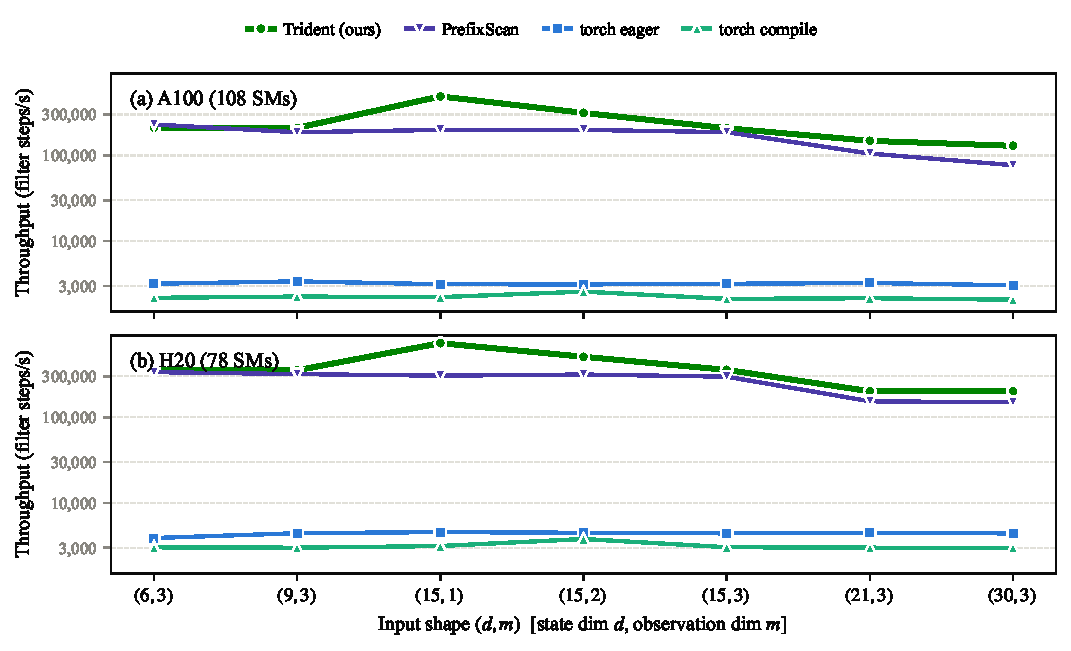
\includegraphics[width=\textwidth]{figures/5-eval-shape.pdf}
  \caption{Throughput of the linear Kalman core as the state dimension $d$ and observation dimension $m$ vary (single trajectory, fp32). (a) A100; (b) H20.}
  \label{fig:shape-compare}
\end{figure*}

On a single trajectory, the fused implementation removes the latency bound that dominates the eager baselines (measured on the H20). The CPU eager fp64 reference sustains $1{,}866$ steps/s; a CUDA Graph replay of the same per-step kernels reaches $2{,}640$ steps/s ($1.41\times$), and whole-scan fusion in fp64 raises this to $16{,}491$ steps/s ($8.8\times$ over the CPU). Switching the fused kernel to the adopted fp32 precision plan reaches $242{,}737$ steps/s, $130\times$ over the CPU reference. Batching independent trajectories then scales the same kernel to $1.9\times10^{7}$ steps/s at 78 trajectories and to a peak of $4.63\times10^{7}$ steps/s at 312 trajectories, approximately $2.5\times10^{4}\times$ the CPU; \Cref{subsec:ablation} analyzes this scaling in detail.

\Cref{fig:shape-compare} generalizes the comparison beyond the end-to-end workload by sweeping the state dimension $d$ and observation dimension $m$ of the linear Kalman core on both GPUs. Two observations hold across the entire sweep. First, the two scan-based implementations outperform the per-step baselines by about two orders of magnitude at every configuration: \texttt{torch eager} and \texttt{torch compile} remain in a narrow $2$--$4.5\times10^{3}$ steps/s band regardless of shape, because their cost is dominated by kernel dispatch rather than arithmetic. Second, \textsc{Trident} is more robust than \textsc{PrefixScan} to both shape directions. Increasing $d$ from 15 to 30 reduces \textsc{PrefixScan} from $1.87\times10^{5}$ to $7.7\times10^{4}$ steps/s on the A100, while \textsc{Trident} retains $1.29\times10^{5}$ steps/s; the H20 panel shows the same ordering. Decreasing $m$ widens the gap in \textsc{Trident}'s favor---at $(d,m)=(15,1)$ it reaches $4.9\times10^{5}$ steps/s on the A100 and $7.3\times10^{5}$ steps/s on the H20, up to $2.3\times$ the corresponding \textsc{PrefixScan} rate---because the analytical innovation inverse removes the cuSOLVER call that the prefix scan requires at every step.

\subsection{Numerical Accuracy Under Mixed Precision}
\label{subsec:precision-evaluation}

We evaluate accuracy on complete trajectories rather than isolated filter steps, because \Cref{subsec:motivation-precision} shows that rounding in recurrent quantities accumulates over the full horizon and a truncated run would understate it. \Cref{tab:precision-fidelity} scores the baselines on the linear Kalman core against a sequential fp64 evaluation of the same filter. All fp32 implementations reproduce that reference to about $10^{-7}$ at the final state, and \textsc{Trident} is the fastest while matching the eager baseline's accuracy grade: $1.8\times$ the \textsc{PrefixScan} throughput and $130\times$ the eager baseline at the same $10^{-7}$ accuracy. Their throughput differences therefore do not come at the cost of accuracy. The only unattractive choice is the TF32 dot product, which degrades by four orders of magnitude to $1.3\times10^{-3}$, confirming the component-aware selection of IEEE dot products in \Cref{subsec:mixed-precision}.

The same ordering holds on the end-to-end SINS/EKF workload, where the filter's own positioning error provides a physical accuracy scale: the adopted fp32 plan deviates from the fp64 CPU reference by only $4.3$\,mm over the complete trajectory---two orders of magnitude below the reference's own $1{,}017.838$\,mm error---while running $130\times$ faster, and the fused fp64 variant deviates by $0.31$\,mm, so the residual error stems from the precision plan rather than from fusion. Applied with the acceptance ratio $\alpha{=}10^{-2}$, the criterion \Cref{eq:precision-accept} admits precision-induced deviations up to $\alpha\,\varepsilon_{\mathrm{model}}\approx10.2$\,mm for this workload---over twice the adopted plan's $4.3$\,mm---so the selection is comfortably within tolerance. Acceleration therefore does not cost accuracy on either workload.

\begin{table}[!t]
  \centering
  \caption{Accuracy and throughput of fp32 implementations on the linear Kalman core, $(d,m)=(15,3)$, single trajectory (A100). $\Delta$ is the final-state deviation $\max|\mathbf{x}-\mathbf{x}^{\mathrm{ref}}|$ from a sequential fp64 evaluation of the same filter.}
  \label{tab:precision-fidelity}
  \begin{tabular}{@{}lrr@{}}
    \toprule
    Implementation & Steps/s & $\Delta$ vs fp64 ref. \\
    \midrule
    \texttt{torch eager} & 2,108 & $1.1\times10^{-7}$ \\
    \textsc{PrefixScan} & 152,932 & $3.0\times10^{-7}$ \\
    \textsc{Trident} (ours) & \textbf{274,428} & $\mathbf{1.2\times10^{-7}}$ \\
    \bottomrule
  \end{tabular}
\end{table}

\subsection{Ablation Study}
\label{subsec:ablation}

We decompose the end-to-end gain of \Cref{subsec:end-to-end} into the three axes of \textsc{Trident} and quantify each axis independently. We first ablate the three contributions against the end-to-end workload, then present Nsight profiling of GPU utilization that connects the observed performance regimes to how the device is actually occupied.

\subsubsection{Axis combination and isolation}
\Cref{fig:ablation-shape} isolates each of the three axes against the eager fp64 GPU baseline on the end-to-end SINS/EKF workload and contrasts them with the full combination. Two observations stand out. First, no single axis suffices: enabling only the fp32 precision plan barely moves the launch-bound eager step ($449\to492$ steps/s), and even batching 108 eager trajectories ($4.4\times10^{4}$ steps/s) loses to a \emph{single} fused fp64 trajectory ($7.1\times10^{4}$ steps/s), because launch-bound execution never reaches the arithmetic that precision or fusion would accelerate. Second, the axes compose multiplicatively rather than additively---fusion $157\times$, precision a further $1.8\times$ on A100, batching $109\times$, whose product ($\approx3.1\times10^{4}\times$) matches the full combination---because each removes a distinct bottleneck: fusion removes dispatch and recurrent-state traffic on the serial critical path, precision shortens per-step arithmetic, and batching fills the SMs a single scan leaves idle. The remaining cells of the $2{\times}2{\times}2$ factorial (measured but omitted from the figure for clarity) confirm that these factors are consistent across conditionings: fusion gains $157$--$311\times$ (rising once the other axes expose arithmetic to it), precision pays only on fused execution ($1.8\times$ at $B{=}1$, $1.24\times$ at $B{=}108$) and is within noise on eager variants, and batching contributes $89$--$157\times$ in every conditioning. Launch-bound variants are invariant to trajectory length, so these conclusions do not depend on the horizon $N{=}166{,}667$.

\begin{figure}[!t]
  \centering
  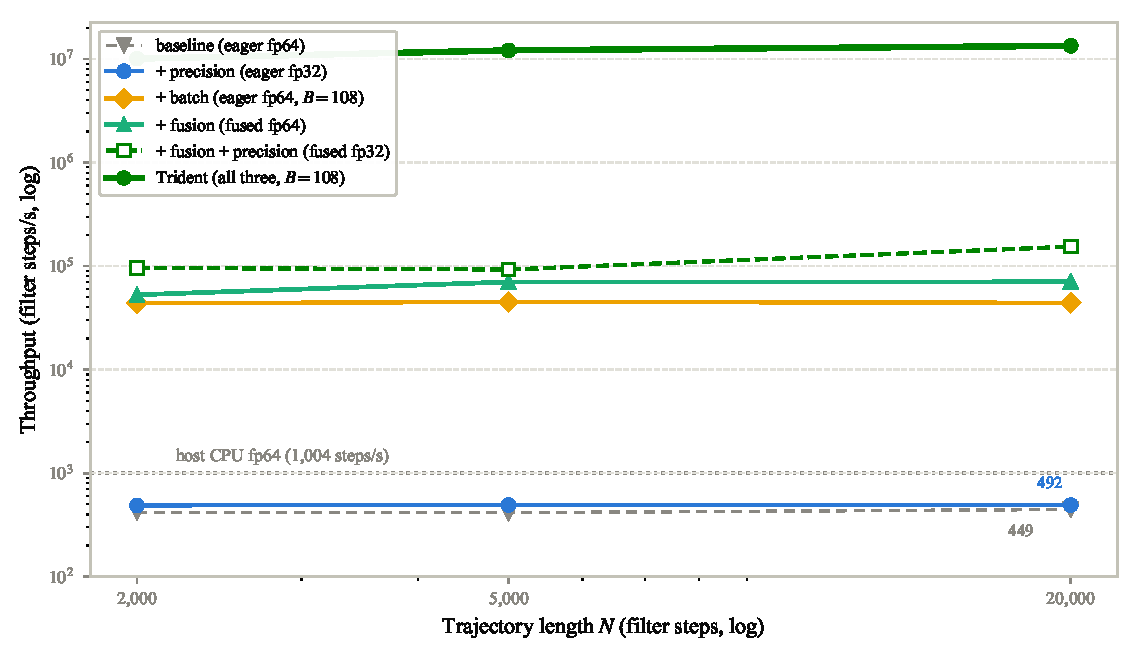
\includegraphics[width=\linewidth]{figures/5-eval-ablation-a100.pdf}
  \caption{Contribution ablation on the end-to-end SINS/EKF workload (A100). Against the eager fp64 GPU baseline, each intermediate series enables exactly one optimization axis in isolation---fusion (fused fp64), the fp32 precision plan (eager fp32), or trajectory batching (eager fp64, $B{=}108$, one per SM)---and \textsc{Trident} enables all three. Because launch-bound implementations are trajectory-length invariant (flat in $N$), all series are shown up to the common horizon $N{=}20{,}000$.}
  \label{fig:ablation-shape}
\end{figure}

\subsubsection{Conditional per-axis gains}
Each axis also carries a caveat that makes its gain conditional rather than automatic. For fusion, the eager tensor port is \emph{slower than the CPU} (263--610 steps/s across $\sim$531 launches per step) and even CUDA Graph replay reaches only $1.41\times$; only enclosing the whole scan in one kernel breaks the latency bound, and a library-composition bound explains why---a cuBLAS $\mathbf{F}\mathbf{P}\mathbf{F}^{\mathsf T}$ plus a cuSOLVER $3\times3$ inverse already cost $2.2\times$ the complete fused step. For precision, the $14.7\times$ on H20 versus only $1.8\times$ on A100: the A100 runs fp64 at half its fp32 rate, so the fp32-over-fp64 ceiling is near $2\times$, whereas on the H20 the fp64 datapath is only a small fraction of the fp32 rate, releasing far greater step-level throughput on the same switch---an asymmetry that motivates the per-device selection of \Cref{subsec:mixed-precision}. The gain on both devices comes from the \emph{selective} assignment: a uniform TF32 plan is both slower ($0.86\times$) and less accurate ($4.82$\,mm) than the adopted fp32/IEEE plan. For batching, \Cref{tab:ablation-batch} shows throughput peaks at $B{=}312$---one full register-limited wave, $186\times$ a single trajectory---and \emph{falls} $24\%$ at $B{=}400$ once wave quantization leaves the second wave only $28\%$ populated, exactly as the register-residency model of \Cref{subsec:batch-parallelism} predicts.


\begin{table}[!t]
  \centering
  \caption{Batch-size sweep of the fused fp32 kernel on H20 (median of repeated runs). Blocks/SM is $B/78$; per-trajectory efficiency normalizes throughput to $B\times$ the $B{=}1$ rate. The $B{=}1$ row corresponds to the fused fp32 configuration of \Cref{subsec:end-to-end}, re-measured as the median of the batch sweep.}
  \label{tab:ablation-batch}
  \begin{tabular}{@{}rrrrl@{}}
    \toprule
    $B$ & Blocks/SM & Steps/s & Efficiency & Regime \\
    \midrule
    1 & 0.01 & 248,159 & 1.000 & linear \\
    8 & 0.10 & 1,959,084 & 0.987 & linear \\
    32 & 0.41 & 7,830,144 & 0.986 & linear \\
    78 & 1.00 & 19,086,444 & 0.986 & one block per SM \\
    96 & 1.23 & 19,954,522 & 0.838 & register co-residency \\
    156 & 2.00 & 32,239,540 & 0.833 & register co-residency \\
    256 & 3.28 & 38,029,702 & 0.599 & register co-residency \\
    312 & 4.00 & 46,290,218 & 0.598 & peak, one full wave \\
    400 & 5.13 & 35,016,136 & 0.353 & oversubscribed \\
    \bottomrule
  \end{tabular}
\end{table}

\subsubsection{Device-utilization profile}
A GPU-utilization profile ties these regimes to how the device is occupied, and \Cref{tab:ablation-profiling} summarizes the measured Nsight counters. Kernel-launch tracing (Nsight Systems) confirms that whole-scan fusion removes the dispatch bottleneck entirely---a full $166{,}667$-step trajectory executes as a single \texttt{ekf\_mega\_kernel\_p} launch---so with no dispatch overhead left, the remaining lever is how much of the device that one launch occupies. Nsight Compute shows the answer for a single trajectory is "very little": one $128$-thread block (four warps) lands on one of $78$ SMs ($\approx1.3\%$ of the device), achieved occupancy on that SM is $6.25\%$ ($4$ of $64$ warps), and device-wide SM throughput is $0.27\%$ (\Cref{tab:motivation-utilization}). This double under-subscription---few SMs among many, few warps within the active one---is the quantitative root of the latency-bound behavior.

\subsubsection{Register-limited batch scaling}
Batch-level mapping closes exactly this gap. At $B{=}78$ the grid places one block on every SM and measured SM throughput rises $74\times$, from $0.27\%$ to $19.91\%$, while per-SM occupancy stays at $6.25\%$ because each SM still hosts a single block. Further residency is bounded by the register file: at $110$ registers per thread at most four blocks are resident per SM, capping theoretical occupancy at $25\%$ and setting the saturation point $B_{\mathrm{sat}}\approx78\times4=312$ measured in \Cref{tab:ablation-batch}. Even at the $B{=}312$ peak occupancy remains register-limited at $25\%$, so the workload is still latency-bound---throughput scales by adding independent recurrences across SMs rather than by filling each SM's pipeline, which is precisely the behavior the batch axis of \Cref{subsec:batch-parallelism} is designed to exploit.

\begin{table}[!t]
  \centering
  \caption{Nsight Compute utilization for the fused fp32 kernel on H20 (64 warps/SM). The single-trajectory row matches \Cref{tab:motivation-utilization}; batching fills SMs without raising per-SM occupancy, which is register-limited to four blocks.}
  \label{tab:ablation-profiling}
  \begin{tabular}{@{}lrr@{}}
    \toprule
    Metric & $B{=}1$ & $B{=}78$ \\
    \midrule
    Grid (blocks) & 1 & 78 \\
    SMs hosting a block & 1 of 78 & 78 of 78 \\
    Device SM throughput & 0.27\% & 19.91\% \\
    Achieved occupancy per SM & 6.25\% & 6.25\% \\
    Registers per thread & 110 & 110 \\
    Resident-block limit (registers) & 4 / SM & 4 / SM \\
    Theoretical occupancy ceiling & 25\% & 25\% \\
    \bottomrule
  \end{tabular}
\end{table}

\subsection{Overhead Analysis}
\label{subsec:overhead}

Mixed precision in \textsc{Trident} is realized inside the fused kernel: input storage ($\mathit{DT}_{\mathrm{IO}}$), recurrent arithmetic ($\mathit{DT}$), and dot-product mode ($\mathit{IP}$) are assigned independently, and each combination is fixed at compile time as a branch-free specialization (\Cref{subsec:mixed-precision}). The dispatch count is unaffected---a trajectory still executes in one launch under any plan---but the number of kernels that must be compiled is not: the current implementation instantiates three plans (fp64, fp32, and TF32), each a separate binary. \Cref{tab:overhead-compile} prices what the protocol of \Cref{subsec:experimental-setup} defers by excluding compilation from all reported timings. A cold start---the first launch with an empty on-disk Triton cache---costs $4.4$\,s for fp64, $2.9$\,s for fp32, and $3.6$\,s for TF32, about $11$\,s for the three specializations together; the cache serves all later launches, so within one device and toolchain the cost does not recur.

\subsubsection{Per-device recalibration}
The cost that does recur is calibration, because both the binaries and the \emph{outcome} of plan selection are device-specific. The acceleration of fp32 over fp64 is $1.8\times$ on the A100 but $14.7\times$ on the H20, and TF32 dot products buy about $3\%$ throughput at a measurable accuracy cost on the A100 while running \emph{slower} than IEEE on the H20; an archive of decisions made on one GPU therefore does not transfer to another. Recalibrating a new device requires recompiling the candidate kernels ($\approx11$\,s), screening each plan with a full-horizon accuracy probe ($1.4$--$2.4$\,s per run), and the fp64 CPU reference trajectory ($\approx163$\,s), which depends on the dataset rather than the device and can be cached and shared across machines. The device-attached part is under half a minute of GPU time.

\subsubsection{Amortization and scope}
This overhead is one-time and amortizes with deployment scale. A single $166{,}667$-step fp32 trajectory executes in about $0.7$\,s at the reported single-trajectory rate, so only one-shot, single-trajectory use is compile-dominated; the multi-trajectory simulation campaigns this workload targets amortize the sub-minute charge over thousands of runs and parameter sweeps. The remaining overheads are conditional rather than systematic---the register-resident state pays a step cost only beyond the $d{=}15$ design point, and block-per-trajectory mapping wastes a partial wave only for batches that are not multiples of $B_{\mathrm{sat}}$ (\Cref{subsec:ablation})---and neither accumulates with the number of deployments. Per-device selection therefore remains practical, which is the same conclusion \Cref{subsec:ablation} reaches from the accuracy side, restated here as a bounded deployment cost.

\begin{table}[!t]
  \centering
  \caption{One-time cost of compile-time precision specialization, measured on the A100. Compilation is a cold start (first launch with an empty on-disk Triton cache) minus an identical warm rerun of the full $166{,}667$-step execution, which isolates JIT compilation; probes are one full-horizon run per candidate plan.}
  \label{tab:overhead-compile}
  \begin{tabular}{@{}L{75pt}R{52pt}L{45pt}@{}}
    \toprule
    Item & Cost & Paid \\
    \midrule
    Kernel compilation, fp64 / fp32 / TF32 & $4.4$ / $2.9$ / $3.6$\,s ($\approx11$\,s) & per device, per plan \\
    Accuracy probe per candidate plan & $1.4$--$2.4$\,s per full run & per device \\
    fp64 CPU reference trajectory & $\approx163$\,s & per dataset (cacheable) \\
    \midrule
    Device-attached subtotal & $<30$\,s & per new device or toolchain \\
    \bottomrule
  \end{tabular}
\end{table}

\section{Related Work}
\label{sec:related-work}

\subsection{GPU-Accelerated Kalman Filtering}
\label{subsec:related-kalman}

GPU implementations of Kalman filtering expose parallelism at several different levels. Early work mapped the matrix operations within a filter step to CUDA and reported speedups when the matrices were large enough to amortize data movement and kernel-launch costs~\cite{huang2011gpu-kalman}. Application-specific systems more often exploit independent estimation problems. The GPU track-fitting implementation of Ai et al.~\cite{ai2021gpu-kalman} processes many particle tracks concurrently, while FastTrack parallelizes the prediction and update of multiple tracked objects and integrates the filter with the surrounding tracking pipeline~\cite{liu2024fasttrack}. These designs are effective when a workload supplies many simultaneous filters, although they do not remove the recurrence or fine-grained execution overhead of one long, small-state trajectory.

Another line of work derives temporally parallel filtering and smoothing algorithms. S\"arkk\"a and Garc\'ia-Fern\'andez formulate Bayesian smoothing operations as associative elements, enabling prefix-scan algorithms with logarithmic span~\cite{sarkka2021temporal}. Such reformulations are attractive when the model admits associative composition and minimizing single-trajectory latency is the primary goal. The downhole traction robot positioning simulation studied here retains the original nonlinear SINS propagation, measurement selection, error feedback, and covariance recursion in their program order. We shorten this sequential path by fusing the complete scan and keeping its recurrent state local, then use independent simulation trajectories---rather than time steps from one trajectory---to occupy the GPU.

\subsection{MegaKernel and Kernel Fusion}
\label{subsec:related-fusion}

Kernel fusion combines operations so that intermediate values can remain on chip and repeated kernel launches can be avoided. MegaKernels enlarge this scope to a substantial computation region; for example, Jia et al.~\cite{jia2020megakernels} place the stages of fast convolution in one GPU kernel to reuse intermediate data and reduce launch and synchronization overhead. Recent compiler and systems research has extended fusion beyond manually selected, memory-bound operator chains. Welder constructs a tile graph to jointly search fusion and tile schedules according to memory traffic~\cite{shi2023welder}. Chimera uses an analytical model to select fusion plans for compute-intensive operators~\cite{zheng2023chimera}, and MCFuser combines memory-bound operators with compute-intensive operators while controlling recomputation and synchronization costs~\cite{zhang2024mcfuser}. These systems show that profitable fusion depends on both the operator graph and the hardware cost created by a candidate fused region.

More recent systems search larger transformation spaces. Mirage represents tensor programs at kernel, thread-block, and thread levels, allowing its superoptimizer to combine algebraic transformations, schedules, and custom-kernel generation~\cite{wu2025mirage}. STOF uses compilation templates and a two-stage search to select adaptive fusion strategies for sparse Transformer inference~\cite{dai2026stof}. These approaches primarily optimize tensor graphs whose operators retain substantial spatial parallelism. Our target presents a different fusion boundary: a complete sequential SINS/EKF trajectory is compiled as one Triton program~\cite{triton}, and its small navigation state and covariance remain program-local across time steps. Parallelism is recovered across independent trajectories, while fusion reduces the latency of each recurrent scan. This specialization complements graph-level fusion systems by addressing a long-lived kernel with an unavoidable loop-carried dependency.

\subsection{Mixed Precision for Scientific Computing}
\label{subsec:related-precision}

Mixed-precision methods have been widely studied in scientific computing and GPU acceleration~\cite{abdelfattah2021survey}. Baboulin et al.~\cite{mixed-precision} combine lower-precision kernels with higher-precision residual evaluation and correction in numerical linear algebra. Haidar et al.~\cite{haidar2018tensorcores} further map low-precision factorization and solves to GPU Tensor Cores while retaining higher precision for accuracy-critical operations.

Automatic precision selection provides a complementary approach. Precimonious searches variable- and operation-level assignments under an application-provided error constraint~\cite{rubio2013precimonious}. CoMP performs operator-wise precision selection for neural-network training through convergence-aware and performance-oriented sampling~\cite{dai2025comp}. Its search also considers format-conversion overhead and the availability of Tensor Core execution, illustrating the importance of evaluating precision plans against both numerical requirements and the characteristics of the target GPU. Unlike these per-operation or per-variable search schemes, \textsc{Trident} fixes one compile-time precision plan per device and validates it over a complete recursive trajectory, so rounding that only emerges over a long horizon is measured before the plan is adopted.

\section{Conclusion}
\label{sec:conclusion}

This paper presents \textsc{Trident}, a three-axis approach to GPU acceleration of SINS/EKF fusion positioning for downhole traction robots. The central observation is that the workload is limited by launch latency, loop-carried dependency, and idle SMs rather than by arithmetic throughput. Whole-scan kernel fusion removes fragmented execution, component-aware precision matches numerical requirements to GPU hardware, and multi-trajectory mapping exposes the independent work needed to fill the device. The resulting implementation turns what is initially a naive GPU slowdown into substantial single-trajectory acceleration and scalable batch throughput: the fused fp32 plan reaches $130\times$ over the CPU reference on a single trajectory, and batching independent trajectories lifts aggregate throughput to roughly $3\times10^{4}\times$ the naive GPU baseline, all while preserving positioning accuracy. Future work will evaluate \textsc{Trident} across additional state-estimation models, trajectory distributions, and GPU architectures, and will investigate structure-aware reductions in covariance computation.

\fontsize{8.5pt}{10pt}\selectfont
\section*{Acknowledgements}
Supported by Frontier Interdisciplinary Exploration Research Program of China University of Petroleum, Beijing (Grant No. 2462024XKQY010).

\input{section/9-competing-interests}

\bibliographystyle{fcs}
\bibliography{references}

% TODO: Add author biographies and high-resolution photographs after the
% author list has been finalized.

\end{document}
